\chapter{Introduction}
\label{chapter:introduction}

\section{General information about \thesistitle}

\thesistitle{} is a software package for modelling strain-/stress-induced rock fabrics and testing the effects of the resulting elastic and viscous anisotropy on seismic imaging and mantle convection patterns. 

\thesistitle{} includes programs for geodynamic modelling (\textbf{ECOMAN-geodynamics}) and seismological modelling (\textbf{ECOMAN-seismology}) that are mostly written in Fortran and Julia language, and where most of the routines are parallelized with a hybrid MPI and OpenMP scheme, providing strong scalability with increasing number of cores.

\textbf{ECOMAN-geodynamics} includes software for (Fig. \ref{fig:flowchart}):
\begin{enumerate}
\item Rock fabrics and mechanical properties simulations:

\begin{itemize}
    \item \textbf{\drexstitle}: Single Aggregate Fabric. This program builds on the original D-REX and estimates the strain-induced LPO of a single mantle aggregate. It includes the necessary \textbf{MTEX Toolbox} libraries to generate pole figures of the (1) LPO and (2) isotropic/anisotropic elastic properties.

    \item \textbf{\drexmtitle}: Multiple Aggregates Fabric. This program builds on the original D-REX and computes the strain-induced LPO of multiple mantle aggregates and output their (1) deformation gradient tensor \textbf{F} and (2) elastic tensor \textbf{C} as a function of the crystals orientation, volume fraction and of the local P-T conditions. 

    \item \textbf{\exevtitle}: this program computes the EXtrinsic Elastic and Viscous anisotropy using Effective Medium Theories (STILWE \citep{backus1962jgr} and DEM (e.g., \citep{mainprice1997tect})). It includes a parametrization of the viscous tensor evolution as a function of the deformation for 2 phases (matrix-inclusion) systems to be used in large-scale mantle convection simulations \citep{demontserrat2021}.


%\item \texttt{Draw.io} -- an online drawing package that can output PDFs to Google Drive -- see \url{https://www.draw.io}.
\end{itemize}

\item Visualisation of the mechanical properties and data formatting in preparation for seismological synthetics:

\begin{itemize}
    \item \textbf{\viztomotitle}: this program processes the \drexmtitle{} output for (1) visualization of the aggregates elastic and deformational history (FSE) properties, and (2) preparing the initial setup for seismic wave propagation simulations (e.g., \textbf{SPECFEM3D},\psitomotitle).
    
    \item \vizvisctitle: this program processes the \drexmtitle{} output for visualization of the aggregates viscous anisotropy and deformational history (FSE) properties.
\end{itemize}

\end{enumerate}

\textbf{ECOMAN-seismology} includes software for seismic forward and inverse modelling:
\begin{itemize}
    \item \textbf{\skstitle}: this program estimates the SKS splitting at a grid of virtual seismic stations placed at the top of the \drexmtitle{} model as a function of the back-azimuth using \textbf{FSTRACK} \citep{becker2006epsl}.
    
    \item \textbf{\psitomotitle}: this software performs isotropic and anisotropic P- and S- wave travel-time + S-wave splitting intensity inversions on either synthetic elastic models computed with \drexmtitle{} and \viztomotitle{} or with real datasets, and utilizing the method of \citep{vanderbeek2021,vanderbeek2023}. Other inversion methods to be added soon!.
\end{itemize}


\begin{figure}
    \centering
    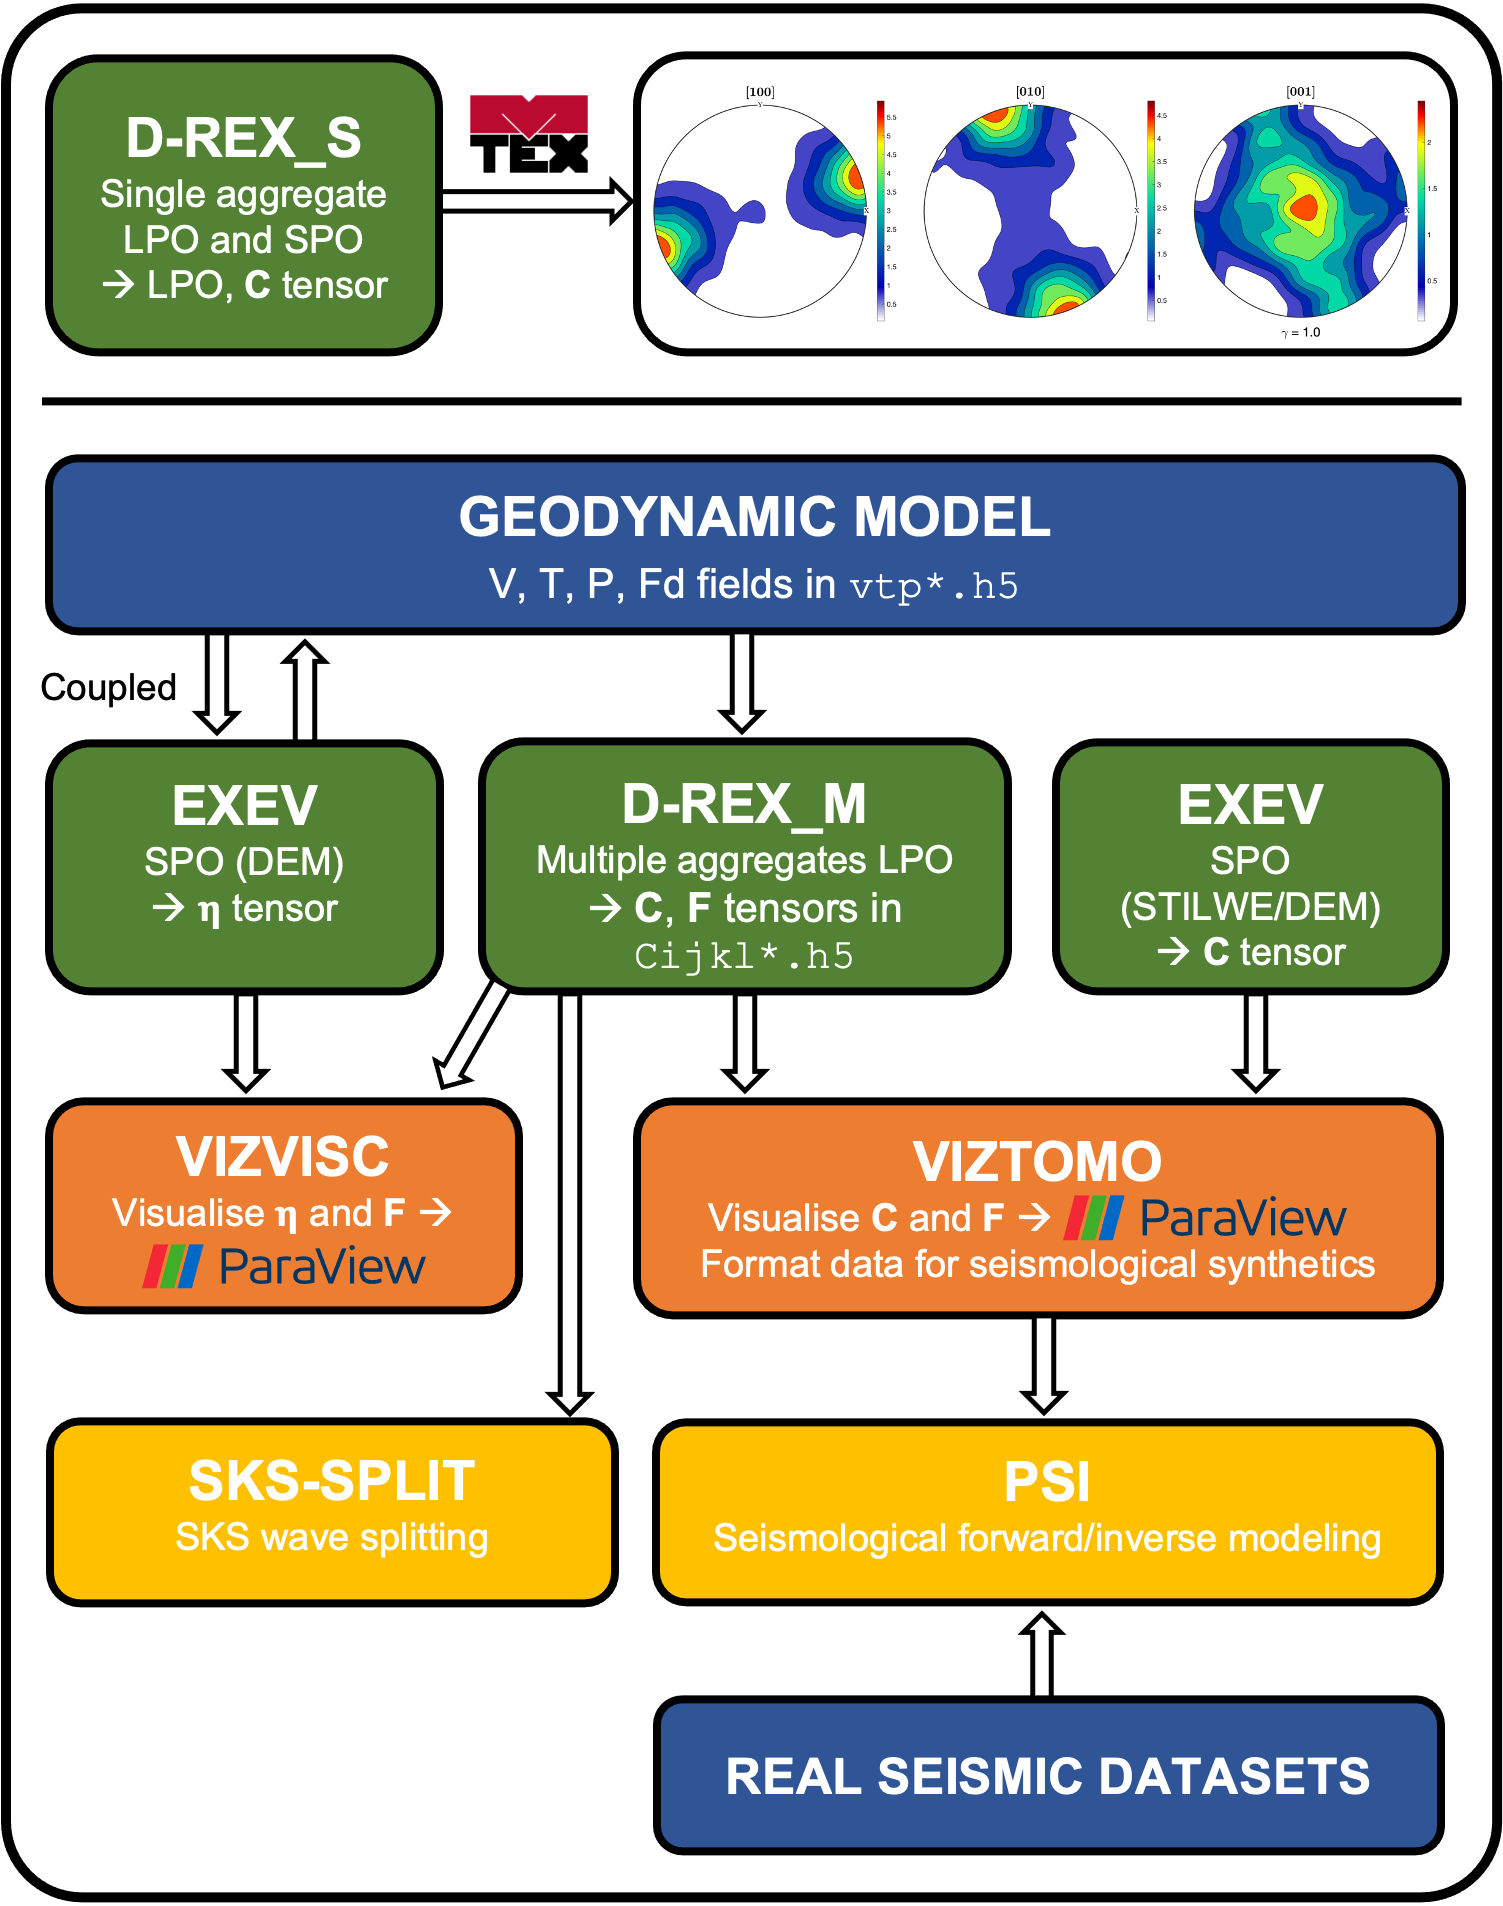
\includegraphics[width=1.0\textwidth]{introduction/FlowChartnew.png}
    \caption{\thesistitle{} structure and flow chart. Coloured boxes denote programs that compute rock fabrics (green), post-process the elastic (\textbf{C}), viscous ($\pmb{\eta}$) and deformation gradient (\textbf{F}) tensors for visualisation and/or data formatting for seismological synthetics (orange), perform seismological forward/inverse modelling on synthetic or real datasets (yellow).  Input data are from geodynamic modelling or real seismic datasets (blue). Visualisation of the mechanical properties and LPO can be done with the MTEX MATLAB toolbox for single crystal aggregates or the software Paraview for large-scale simulations.}
    \label{fig:flowchart}
\end{figure}

\section{Why \thesistitle?}
The understanding of the Earth’s interior is mainly based on seismological and geodynamic modelling, the first one providing important information about the present-day structure, while the second about the Earth’s geological history.
Seismological and geodynamical modelling are typically conducted separately, which creates difficulties in both interpreting seismic data in terms of geodynamic processes and in providing mantle structure constraints to geodynamic models.
From this perspective, \thesistitle{} aims at linking seismology and geodynamics by providing a set of software to estimate the mantle elastic properties as a function of the deformation history and local P-T conditions. The modelled elastic properties can be used to generate tomographic models and run forward/inverse seismological problems (as it is done with real datasets), and the output compared with observations. \\
In addition, \thesistitle{} allows estimating the role of extrinsic viscous anisotropy in large-scale mantle convection models by providing a parametrization of the strain-induced evolution of the SPO-related fabrics in two-phase (matrix-inclusions) systems.

When compared to other similar softwares/packages, \thesistitle:
\begin{itemize}
    \item aims at being a more versatile package suitable for any geodynamic simulations (2D/3D  cartesian/polar coordinate systems; regional/global settings),
    \item takes into account for the time-dependent deformational history of the mantle (which is usually not steady-state, especially close to plate boundaries),
    \item predicts the strain-induced fabric and elastic tensor of different mantle layers (i.e., not only the upper mantle),
    \item includes Effective Medium Theories (STILWE, DEM) and a parametrization of the fabric evolution of 2-phase composites to predict extrinsic elastic and viscous anisotropy, 
    \item generates realistic grid structures distributions of mantle elastic properties to be used for forward/inverse seismological modelling (e.g., \textbf{SPECFEM3D}, \psitomotitle).  
    \item performs synthetic seismic inversions (e.g., P- and S-wave travel-time tomographies, S-wave splitting intensities) within the computational domain, which facilitates the comparison with other tomographic models and the estimation of apparent anomalies (artefacts) due to, for example, unaccounted-for elastic anisotropy (\citep{bezada2016g3,vanderbeek2021,vanderbeek2023}) and/or regularisation. 


\end{itemize}

\section{Referencing and useful links}
If you use \thesistitle{}, please cite one of the following paper that best fits your application.

\begin{enumerate}
    \item New paper about \thesistitle{} (Faccenda et al., submitted)
    \item \citep{faccenda2013g3}: \drexmtitle{} methodology explained in detail; applied to upper mantle fabrics.
    \item \citep{faccenda2014pepi}: Extension of \drexmtitle{} to mantle fabrics of the MTZ and ULM; elastic tensors scaled by local P-T conditions.
    \item \citep{bezada2016g3}: First example of synthetic P-wave travel-time tomography on mantle fabrics generated with \drexmtitle.
    \item \citep{hu2017EPSL}: \drexmtitle{} goes spherical.
    \item \citep{faccenda2019JGR}: Evaluation of extrinsic elastic anisotropy in mantle aggregates.
    \item \citep{ferreira2019natgeo}, \citep{sturgeon2019g3}: Evaluation of lower mantle intrinsic and extrinsic fabrics to explain the observed seismic anisotropy.
    \item \citep{vanderbeek2021,vanderbeek2023}: Isotropic and anisotropic tomography with \psitomotitle{} on mantle fabrics generated with \drexmtitle.
    \item \citep{demontserrat2021}: submitted, viscous anisotropy due to extrinsic fabrics.
\end{enumerate}

\vspace{0.5cm}
Useful references and links:\\*

\textbf{\thesistitle{}} download: \url{https://github.com/ecoman-geos} \\* 

\textbf{\thesistitle{}} website: \url{https://newtonproject.geoscienze.unipd.it/ecoman/} \\*

\textbf{D-REX}: \url{http://www.ipgp.fr/~kaminski/} \citep{kaminski2004gji}\\*

\textbf{FSTRACK}: \url{https://github.com/thwbecker/fstrack} \citep{becker2006epsl}\\*

\textbf{MTEX Toolbox}: \url{https://mtex-toolbox.github.io/index.html} \citep{mainprice2011gsl}\\*

\textbf{\mmaeostitle{}}: \url{https://bitbucket.org/chust/eos} \citep{chust2017jgr}

\section{Author contribution}
\thesistitle{} was developed by Manuele Faccenda (geodynamic modelling and visualization), Brandon P. VanderBeek (developer of \psitomotitle{} module and of body-wave anisotropic inversion method), with fundamental contributions by Albert de Montserrat (derived and tested the parametrization of the extrinsic viscous anisotropy) and Jianfeng Yang (testing and applications). 

\section{Acknowledgements}
The development of \thesistitle{} has been funded by the ERC StG 758199 NEWTON and the Università di Padova FACCPRAT12 granted to Manuele Faccenda.